\documentclass[acmtog, authorversion]{acmart}
\usepackage[htt]{hyphenat}
\usepackage{graphicx}
\usepackage{lipsum}
\usepackage{pgfgantt}
\usepackage{enumitem}
\usepackage{booktabs}
\usepackage{fontawesome5}

\newlist{questions}{enumerate}{2}
\setlist[questions,1]{label=\textbf{RQ\arabic*.},ref=RQ\arabic*}
\setlist[questions,2]{label=(\alph*),ref=\thequestionsi(\alph*)}
\graphicspath{{images/}}

\AtBeginDocument{%
  \providecommand\BibTeX{{%
    \normalfont B\kern-0.5em{\scshape i\kern-0.25em b}\kern-0.8em\TeX}}}

\setcopyright{cc}
\copyrightyear{2023}
\acmYear{2023}

\acmConference[TScIT 39]{39$^{th}$ Twente Student Conference on IT}{July 8,
  2023}{Enschede, The Netherlands}

\acmCodeLink{https://github.com/repository/code}


\begin{document}

\title{Satellite to Radar: Sequence to Sequence Learning for precipitation nowcasting}

\author{Mark Bruderer}
\email{m.a.bruderervanblerk@student.utwente.nl}
\affiliation{%
  \institution{University of Twente}
  \streetaddress{P.O. Box 217}
  \city{Enschede}
  \country{The Netherlands}
  \postcode{7500AE}
}

\renewcommand{\shortauthors}{Mark Bruderer}

\begin{abstract}
\section*{Abstract}
The forecasting of rain is a complex problem with centuries of scientific work. The implications of weather for individuals and companies continue to be important. Machine Learning approaches have been shown to outperform state of the art physics based models of weather for short term predictions. We introduce a new type of model \textbf{Sat2Rad}. Our model takes as input multi-spectral satellite data and outputs radar reflectivity at a set of time-steps ranging from 15 to 180 minutes in the future. This model is novel for precipitation nowcasting because it uses several satellite spectral bands instead of using radar data as input.
\end{abstract}

\keywords{Machine Learning, Sequence to Sequence, Radar, Satellite, Storms, Forecasting}

\settopmatter{printacmref=false}

\begin{teaserfigure}
  \includegraphics*[width=\textwidth, trim=0in 0.0in 0in 16.0in]{images/lightning.jpg}
  \caption{A supercell thunderstorm at twilight in SW Oklahoma.}
  \Description{A supercell thunderstorm at twilight in SW Oklahoma.}
  \label{fig:teaser}
\end{teaserfigure}

\maketitle

\section{Introduction} \label{introduction}

Precipitation forecasting is essential to reduce the risk of life threatening situations. Different types of rainfall ranging from mist to heavy rain have a major impact for different societal sectors including agriculture, aviation, outdoor events, and the energy industry.
By having timely and accurate predictions of rainfall which in turn indicate the potential for destructive storms we can prevent injuries, assist companies in predicting energy production and use resources efficiently.
\medskip

% Predicting and understanding weather has become crucial in a number of industries, including agriculture, autonomous driving, aviation, or the energy sector. For example, weather conditions play a significant role for aviation and logistics companies in planning the fastest and safest route. Similarly, renewable energy companies need to be able to predict the amount of energy they will produce at a given day. As a consequence various weather models have been developed and are being applied all over the world. Unfortunately, these models often require highly specific information about the atmosphere and exact conditions.

% explain what storms are:
% - why are storms important
% - what are storms => how they from
A particularly strong threat is posed by rain storms and thunderstorms. Storms are one of the most destructive weather events in nature, capable of destroying human structures and even lead to loss of life \cite{noaa-national-severe-storms-laboratory-no-date}. Predicting storms is crucial and presents it's own set of challenges.
\medskip

% explain how to currently predict storms
At present meteorologists are able to successfully predict many instances of precipitation. Techniques that are used in practice range from manual analysis of current weather data (e.g radar or satellite images) to complex physics based simulations of our atmosphere with Numerical Weather Prediction (\textsc{NWP}) models.
Various traditional precipitation nowcasting methods are based on \textit{optical flow}. Optical flow functions in two steps, first cumulonimbus clouds are identified, and then their movement is tracked to predict the location of precipitation. Thus in this the case, the \textit{cell-lifecycle} \cite{noaas-national-weather-service-no-date} is not taken into account \cite{prudden2020review}.
\medskip

% explain machine learning approaches
Machine Learning (\textsc{ML}) approaches have also been developed to predict precipitation. An improvement of machine learning models over \textsc{NWP} models is that they are much faster to produce predictions, thus ML models are more suitable for real-time or near-real-time predictions, such as required in disaster response and energy management. According to the universal approximation theorem \cite{cybenko-1989}, deep neural networks have the property of being able to approximate any function provided they have the correct weights, thus it is suggested that machine learning models can incorporate sources of predictability beyond optical flow such as the cell-lifecycle among others \cite{prudden2020review}.
\medskip

% explain our approach
Thus far most machine learning approaches for precipitation nowcasting have focused on predicting a next frame in a time series of radar reflectivity data \cite{shi2017deep, convlstm, rainet}. However taking this approach may eliminate the possibility of learning the cell-lifecycle, due to the fact that the model only sees precipitation itself but not the cloud that is causing the precipitation.
\medskip

% "Yet the key issue of precipitation prediction – the anticipation of convective initialization, as well as the growth and dissipation of precipitation in the imminent future – still appears to be unresolved" 

We propose to use multi-spectral satellite data to learn spatio-temporal mappings between sequences of satellite data and precipitation data in the near future. If this is successful \textit{cumulonimbus} clouds could be predicted from when they are mere \textit{cumulus} clouds and prior. An additional advantage is that contrary to radar data, satellite data is readily available over oceans and remote communities which allows for the prediction of precipitation over these regions. We will work towards creating a model by answering the following main research question:
\smallskip

% Most physical models are based on the extrapolation of the detected Cbs with atmospheric motion vectors (AMV; see [14] and the references therein). This approach works well as long as the cells do not decay during the prediction period. Unfortunately, cells usually do decay after a certain lifetime, such that this effect occurs regularly. Further, newly developed cells cannot be captured by extrapolation of detected cells. These are serious drawbacks of the AMV approach. The quite good results achieved with deep learning indicate that the training process might enable the network to gain information on the life cycles of cells (decay, newly developed cells). The network seems to be able to learn to a certain extent whether Cbs decay or newly develop within the prediction period or not, and we believe this is crucial for lead times around or larger than 180 min, as the lifetime of regular Cbs is usually shorter than this; see, e.g., 
% - 

% Radar has been the primary tool for predicting precipitation for decades, but it has limitations, such as its limited range and the fact that it cannot penetrate through heavy precipitation. This makes it difficult to predict precipitation in areas that are far from the radar, such as remote regions and over the ocean.

% Satellite data, on the other hand, can provide a global view of weather patterns and can be used to fill in gaps in radar coverage. Satellites can also provide information about cloud temperature, humidity, and other atmospheric conditions that can be used to infer the presence of precipitation. Additionally, satellite data can be useful for predicting the onset and duration of precipitation events, which can be valuable information for planning and emergency response.

% However, using satellite data for precipitation nowcasting also presents some challenges, such as the need to develop accurate algorithms for translating satellite data into precipitation estimates. These algorithms must take into account factors such as the altitude of the clouds, the types of precipitation (e.g. rain, snow, or hail), and the intensity of the precipitation. Despite these challenges, the use of satellite data for precipitation nowcasting shows great promise and has the potential to improve our ability to predict precipitation in a variety of settings.
\subsection{Problem Formulation}
We approach precipitation nowcasting as a
self-supervised problem. A self supervised task arises when
no explicit labels are given, but instead labels can be taken from the raw data itself
as is commonly the case with time-series data.
We can therfore apply known techniques in supervised learning to solve our research problem.
\\

Consider a dataset \{X, Y\} consisting of pairs of input-output sequences indexed by $i \in \mathbb{N}$,
%where each input sequence represents a temporal sequence of $t$ satellite images with height $H$, width $W$ and $c$ channels.
Let $$X = \{\forall i | x^{(i)} \in \mathbb{R}^{t \times H \times W \times c}\}$$
where $x^{(i)}$ is a tensor of dimension $t \times H \times W \times c$ representing the sequence of satellite images at position i, having t timesteps, H height, W width and c channels.
The set of output sequences is denoted as $$Y = \{\forall i | y^{(i)} \in \mathbb{N}^{W\times H}\}$$
where $y^{(i)}$ represents the $i_{th}$ H $\times W$ dimensional tensor containing discrete integers mapping to rainfall intensity classes.

The problem is formulated as finding a probability mass function p(x). This function must minimize the Cross Entropy Loss expressed as follows:

$$E = \frac{1}{H+W}\sum_{i=1}^H\sum_{j=1}^W t_{ij} log(p_{ij})$$

Let $\hat{Y} = \{\forall i | p(x^{(i)})\}$, representing the predicted outputs for each sequence of satellite images and identical in dimensions to $y^{(i)}$.
find p(x) such that $E(\hat{Y}, Y)$ is minimized.




\section{Main Contribution}
This proposal has the potential to contribute a deep learning model capable of predicting precipitation in the short term with only satellite images.

\section{Related Works}

In this section we will discuss the existing work in precipitation nowcasting via machine learning. This section is structured by the type of input data used in the approaches, first we list radar based learning and then we discuss satellite based approaches.

\subsection{Radar Based Nowcasting}

Recurrent neural networks (\textsc{RNNs}) have been created to learn temporal relationships in data, therefore they are a natural candidate to the task of learning spatio-temporal patterns of weather. The \textsc{LSTM} architecture was developed by Hochreiter and Schmidhuber \cite{lstm}, to solve the problem of vanishing and exploding gradients in RNNs and is widely used. Taking LSTM as a base and adapting the weights to kernels, \textsc{ConvLSTM} \cite{convlstm} was introduced for the task of precipitation nowcasting. Multiple layers of ConvLSTM are used in this paper to obtain a sequence to sequence architecture. A further improvement of ConvLSTM is \textsc{trajGRU} which was proposed by Shi et al. \cite{shi2017deep} to be able to learn the \textit{location-variant} structure for recurrent connections.
\medskip

Pure convolutional neural networks have also been used to predict precipitation. As demonstrated by Bai et al. and Gering et al. \cite{bai2018empirical, gehring2017convolutional} convolutional neural architectures can outperform recurrent neural networks for a variety of sequence modelling tasks. This is the reason why many works on precipitation nowcasting have opted for pure convolutional networks \cite{rainet,agrawal2019machine}.
\medskip

Due to machine learning models attempting to minimize loss, \textit{blurry predictions} can be produced by models. This can be alleviated by using generative models which sample from the possible futures and do not seek to provide a best average fit. Generative Adversarial Networks have been successfully applied to the task of precipitation nowcasting \cite{Ravuri_2021}.

\subsection{Satellite Based Nowcasting}

In their study Chen et al. built a \cite{precipitationEstimationFromSat} MLP to forecast radar data from satellite data. The researchers used a combination of low earth orbit satellite passive microwave and infrared channels from two different satellites. Their model is developed to predict up to 1.5 hours in the future by recursive predictions of the model.
\medskip

A study that does not predict precipitation but uses lightning as a marker for extreme precipitation was performed by Brodehl et al. \cite{predictionLightning} this study uses a convolutional network to predict lightning events, and contributes the important observation that both the visual and infrared channels are significant in differing ways to predict lightning.
\medskip

The approach taken by the researchers of MetNet \cite{sønderby2020metnet} is to combine a convolutional block for spatial downsampling, then a ConvLSTM block for temporal encoding and finally a Axial attention block \cite{vaswani2017attention}. MetNet is able to perform more accurate forecasts than NWP models for up to 8 hours. In this study the input data that is used is both satellite and radar data as well as the elevation, time of the year and latitude and longitude values.

\section{Background}
In order to understand this research it is important to be acquainted with the machine learning techniques that will be used. Furthermore insight into this study can be enhanced by having more in depth information on the used data-sets and the meteorological theory.
\medskip

For the machine learning aspect of this research it is important to understand multi layer perceptrons (\textsc{MLPs}) \cite{schmidhuber2022annotated}. Furthermore it is important to understand convoutional neural networks and what benefits they afford in relation to \textsc{MLPs} \cite{oshea2015introduction}. It is also crucial to have an understanding of recurrent neural networks (RNNs) and their extension to include convolutions \cite{convlstm}.
\medskip
\subsection{Convolutional Neural Networks}
Convolutional Neural Networks (CNNs) or Fully Convolutional Networks (FCNs) are a class of deep learning models suited for computer vision tasks. Unlike fully connected neural networks, which treat input data as a one dimensional vector, CNNs are designed to process higher dimensional data such as images.
This distinction enables CNNs to exploit more spatial relationships and patterns in visual data as opposed to a flattend vector where these patters are not recoverable.

CNNs were first introduced by [] in 1987, but were shown to beat state of the art classification with the ImageNet paper.

This ability to automatically extract meaningful features from images is a fundamental advantage of CNNs over fully connected networks, as it significantly reduces the number of parameters and alleviates the computational burden associated with processing high-dimensional inputs. Furthermore, CNNs leverage parameter sharing, enabling them to efficiently learn translation-invariant features across the entire image. These inherent advantages make CNNs particularly effective for computer vision tasks, such as image classification, object detection, and semantic segmentation.
In CNNs, the core building blocks are convolutional layers, pooling layers, and fully connected layers. A typical CNN architecture consists of multiple convolutional layers, each followed by a non-linear activation function, such as ReLU (Rectified Linear Unit), which introduces non-linearity into the network. Convolutional layers perform the convolution operation by applying a set of learnable filters to the input image, producing feature maps that capture local patterns. The pooling layers, commonly implemented as max pooling or average pooling, downsample the feature maps, reducing their spatial dimensions while preserving the most salient information. This downsampling helps achieve translation invariance and improves computational efficiency. The final layers of a CNN usually consist of one or more fully connected layers, which aggregate the learned features and make predictions based on the extracted representations. The parameters of the CNN are optimized through backpropagation and gradient descent algorithms, enabling the network to learn discriminative features that are highly informative for the given task.
The modular architecture and hierarchical nature of CNNs make them well-suited for extracting spatial features from images and effectively capturing the complex patterns present in computer vision tasks. Their ability to automatically learn relevant features from raw pixel data, combined with their parameter sharing and hierarchical structure, has revolutionized the field of computer vision and significantly advanced the state-of-the-art in various visual recognition tasks.

\subsection{Unet}
Semantic segmentation, the task of assigning a class label to each pixel in an image, plays a crucial role in computer vision applications such as image understanding and scene understanding. U-Net, a convolutional neural network (CNN) architecture, has emerged as a highly effective solution for semantic segmentation tasks, providing accurate and detailed pixel-level predictions. The U-Net architecture is specifically designed to address the challenge of limited training data and to capture both local and global context information.
The U-Net architecture gets its name from its U-shaped design, which consists of an encoder path and a decoder path. The encoder path resembles a traditional CNN and serves to capture spatial information and learn feature representations at various scales. It typically comprises multiple convolutional and pooling layers, where each convolutional layer extracts increasingly abstract features by convolving with learnable filters and applying non-linear activation functions.
The decoder path, on the other hand, aims to recover the spatial information lost during the pooling and downsampling operations of the encoder. It employs a series of upsampling and transposed convolutional layers to gradually increase the spatial resolution and reconstruct the detailed predictions. The skip connections between the corresponding encoder and decoder layers help preserve fine-grained details and enable the fusion of local and global context information, facilitating more accurate segmentation. These skip connections bridge the gap between low-level and high-level features, allowing the network to leverage both local and global context for precise pixel-wise predictions.
One of the key advantages of U-Net is its ability to capture contextual information effectively. By using skip connections, the network can combine low-level and high-level features, enabling the model to refine predictions by incorporating local details and global context simultaneously. This property is especially beneficial for tasks like semantic segmentation, where precise boundary delineation and accurate classification of object categories are essential.
Furthermore, U-Net has gained popularity due to its relatively small number of parameters compared to other fully convolutional networks, making it more computationally efficient while maintaining competitive performance. This aspect is particularly advantageous when dealing with limited training data or when deploying models on resource-constrained devices.
In summary, U-Net has emerged as a powerful CNN architecture for semantic segmentation tasks. By leveraging its U-shaped design, skip connections, and an effective combination of local and global context information, U-Net achieves accurate and detailed pixel-wise predictions. Its ability to capture contextual information while being computationally efficient makes it an attractive choice for various computer vision applications requiring fine-grained segmentation.




\subsection{Convolutional Neural Networks}
Why do they exist
motivation for conv nets comes from losing info when flattening but also when processing images it is possible for a pixel to
receive info from all others becomes very expensive $t^2$ but when using conv nets its the kernel that is being learned. image transformation kernels manually developed. Combining the identically
with ANN we can learn the weights of the kernels, for our given problem.

How do they work
they work

\subsection{Recurrent Neural Networks}

\subsection{Convolutional LSTM}

\subsection{Axial Self-Attention}
To have an understanding of the meteorological context of this project it is recommended to have an understanding of radar data \cite{rinehart1991radar}, satellite data specifically the kind used in this project \cite{schmid-no-date}.

\textbf{RQ1}: \textit{How can a deep learning model be trained to predict radar data with multi-spectral satellite data ?}
\smallskip

This research question will be answered by looking at the following sub research questions:
\begin{enumerate}
    \item \textit{what is necessary to build a well performing model ?}
    \item \textit{what methods can be used to create this model ?}
    \item \textit{what is the effectiveness of the trained model ?}
    \item \textit{what are the conditions under which the model can and cannot be used ?}
\end{enumerate}
\section{Methodology}
We choose to structure our project based on the CRISP-DM framework.

\subsection{Business and Data Understanding}
From a business perspective the data.

\subsection{Data Preprocessing}

For the preprocessing of data we created a pipeline which distinguishes between satellite images and radar images to preprocess each following their own needs (See figure \ref{fig:preprocessing}).

In the case of satellite data, we first download this data contained in zip files from a storage bucket. After all files are downloaded they are extracted into zip files, the pipeline takes care of deleting any files which are not needed anymore.
Then we reproject the satellite images using the \texttt{satpy} package. By reprojecting we reduce the dimensions of each satellite image to \texttt{256 x 256} pixels.
Via the reprojection we also obtain only the area of interest. specified by the coordinates for the lower corner (0, 50) and upper corner (1) of the region, this gives us the benelux region. This is the same region as given in the radar data.
Additionally the projection is matched between the satellite image and radar image.
After reprojecting we perform a \textit{statistics} step where we aggregate the dataset by finding the minimum and maximum values for each channel.
The statistics are necessary for the next step which is normalization. During the normalization step we perform the \textit{Min-Max} Normalization (equation 1).

\begin{equation}
  x_{normalized} = \frac{x-min}{max-min}  
\end{equation}

After finalizing the normalization step we sample an image from the dataset which is visualized to check for errors in the pipeline.

The radar pipeline begins with the downloading of radar files in the form of \texttt{h5} files. The collected files are each converted to decibels relative to Z (dBZ) from their previous unit.

\begin{equation}
  dBZ = x \cdot 0.5 - 32
\end{equation}

The preprocessing pipeline then splits into two, one step will normalize values between 0 and 1 using \textit{Min-Max} normalization and the other step will use levels of \textit{dBZ} to create discrete ranges of precipitation to use as classes during training.
Finally the current images in the pipeline are resized using the nearest neighbor algorithm, to avoid changing the values with bilinear interpolation.
Next identically to the satellite pipeline we sample and visualize a radar image for verification purposes.


\begin{figure}
  \centering
  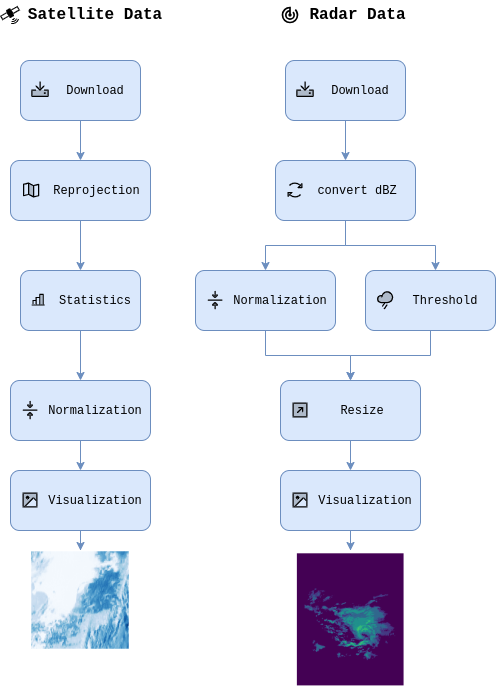
\includegraphics[width=225pt]{./images/preprocessing.png}
  \caption{Preprocessing Pipeline}
  \Description{Satellite Image of the earth}
  \label{fig:preprocessing}
\end{figure}

\subsection{Training}
In order to build and train our models we worked with pytorch. We used pytorch lightning to provide a higher level interface to speed up the research process. To track our experiments we connected pytorch ligthning to mlflow, using MlFlow we can log metrics, atrifacts produced during training while keeping track of the used parameters during that training run.
To create pipelines for preprocesing and training, we used the zenml library.

We created 4 different datasets for our research. These datasets result from the combination of sliding and sequential datasets with class and regression datasets.
We implemented these datasets as subclasses of pytorch vision datasets. We also created time based utility functions to align the start and ending times of satellite data and radar data, such that when data is split based on training, validation and testing percentages, data is still in the same temporal range. Keeping in mind that the radar data has a differnt resolution and is received at a different strides.

\subsection{Performance Evaluation}

Different metrics were used for the regression and the classification.

Classification evaluation metrics:
\begin{enumerate}
  \item Precision
  \item Accuracy
  \item Recall
  \item Exact Match
  \item F1 Score
  \item Jaccard Index
\end{enumerate}

\begin{equation}
  MSE = \frac{\sum (\hat{y_i} -y_i)^2}{n}
\end{equation}

\begin{equation}
MAE = \frac{\sum |\hat{y_i} -y_i|}{n}
\end{equation}

\begin{equation}
RMSE = \sqrt{\frac{\sum (\hat{y_i} -y_i)^2}{n}}
\end{equation}

Additional metrics come from the study \cite{shi2017deep}, where the authors created \textit{B-MSE} and \textit{B-MAE} due to the fact that the frequencies of different rainfall levels are imbalanced. Models trained with conventional \textit{MSE} or \textit{MAE} are biased towards predicting low amounts of precipitation. This can be solved with a loss function that weights the higher precipitation more strongly. The weighting function \textit{w} can be found in the study as well.

\begin{equation}
BMSE = \frac{\sum w(\hat{y_i}) \cdot (\hat{y_i} -y_i)^2}{n}
\end{equation}

\begin{equation}
BMAE = \frac{\sum w(\hat{y_i})  \cdot (\hat{y_i} -y_i)^2}{n}
\end{equation}


\section{Results}


\begin{figure}
    \centering
    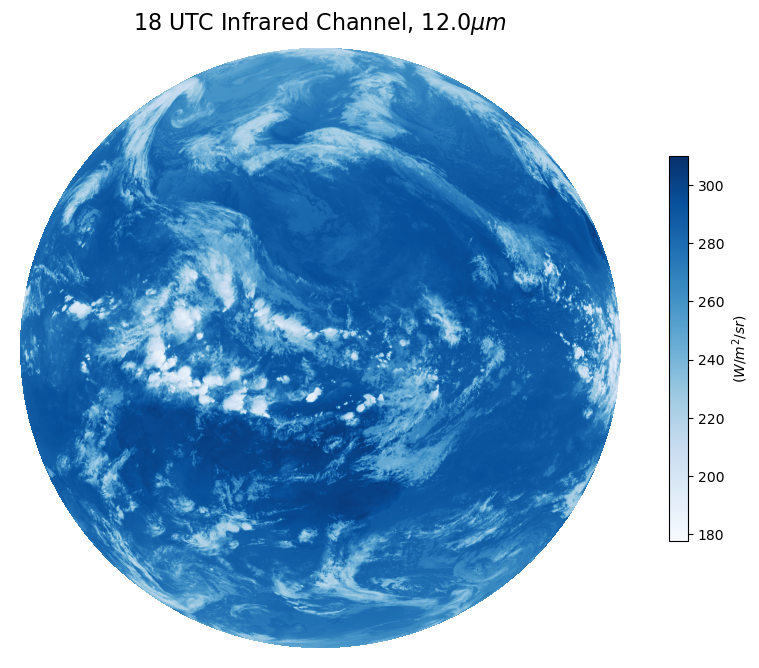
\includegraphics[width=225pt]{./images/infrared.png}
    \caption{Satellite Image: Infrared Channel 18UTC $12.0\mu m$}
    \Description{Satellite Image of the earth}
    \label{fig:infra}
\end{figure}


\section{Conclusions}
At this point in the research we have created an \hyperref[introduction]{introduction for the research}. We have also performed a literature review of available work in the field of precipitation nowcasting. We have written the methods that we will use to perform the research and listed expected results. And we have visualized some of the data from our dataset.

\begin{acks}
I would like to thank my supervisor from Elena Mocanu, for her help. Furthermore I would like to thank I would like to thank Dina Lazorkeno for proofreading my thesis.
\end{acks}

\bibliographystyle{ACM-Reference-Format}
\bibliography{ref}

\newpage
\appendix
%Appendix A
\section{Appendix}

\begin{figure}
    \centering
    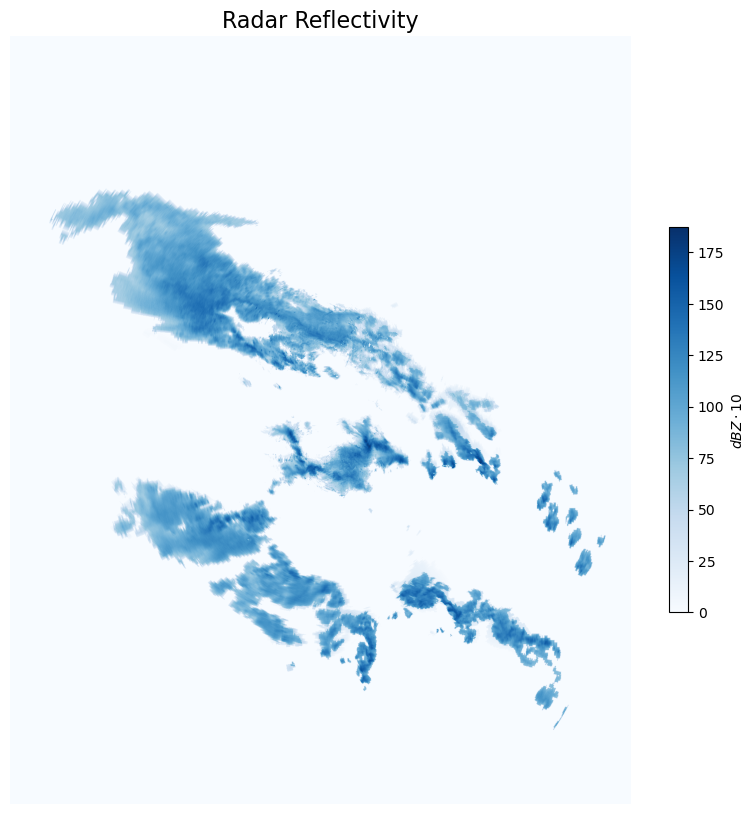
\includegraphics[width=225pt]{./images/radar_reflectivity.png}
    \caption{Radar Reflectivity}
    \Description{}
    \label{fig:reflect}
\end{figure}

\begin{figure}
    \centering
    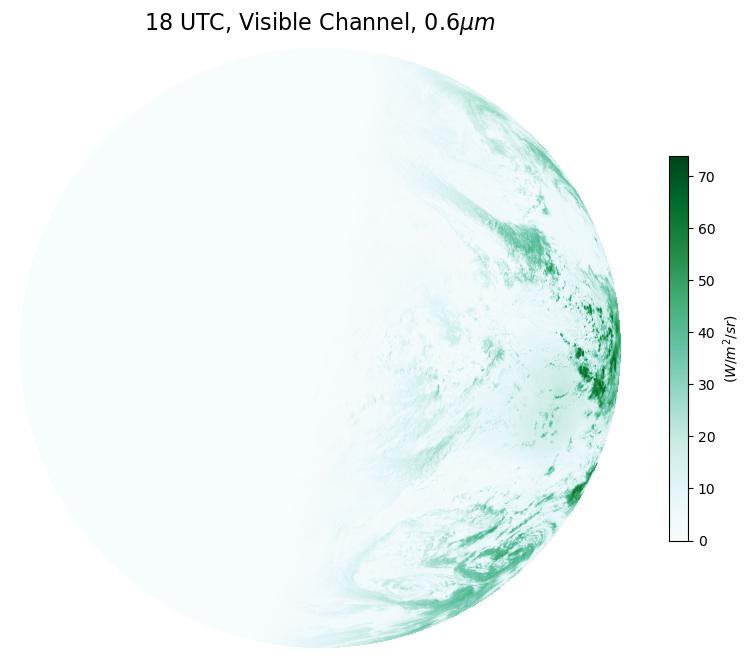
\includegraphics[width=225pt]{./images/vis_006.png}
    \caption{Satellite Image: Visible Channel 18UTC $0.6\mu m$}
    \Description{}
    \label{fig:vis}
\end{figure}

\begin{figure}
    \centering
    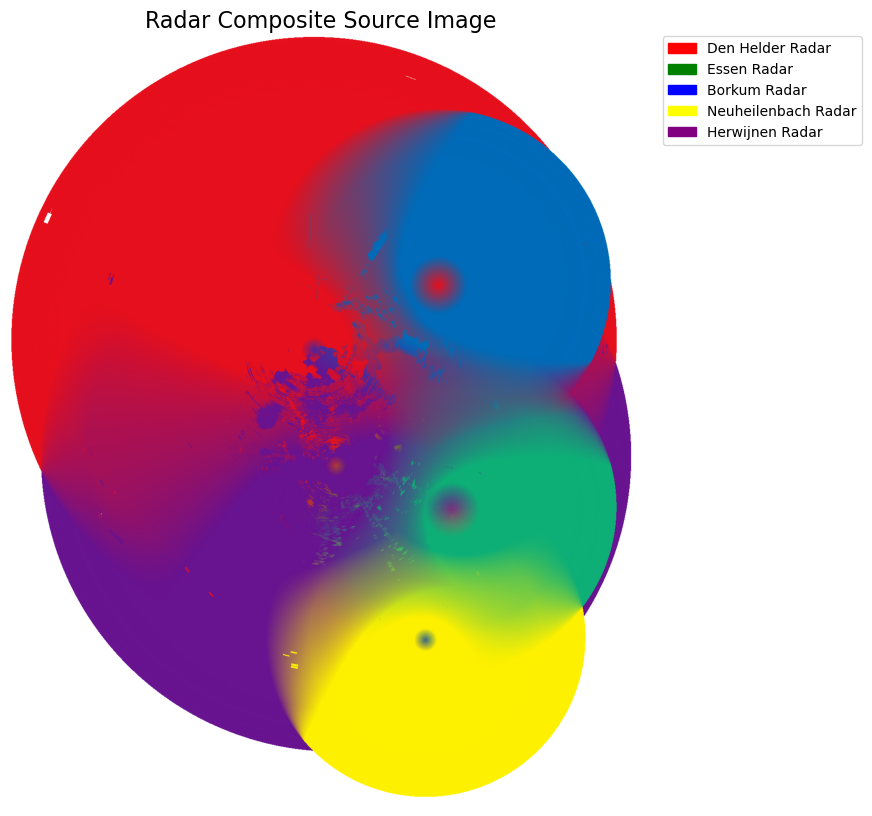
\includegraphics[width=225pt]{./images/radar_source.png}
    \caption{Satellite Image: Infrared Channel 18UTC $12.0\mu m$}
    \Description{}
    \label{fig:source}
\end{figure}


\begin{table}[h]
\caption{Reflectivity in dBZ versus Rainrate}
\begin{tabular}{@{}llll@{}}
\toprule
LZ(dBZ) & R(mm/h) & R(in/h)        & Intensity             \\ \midrule
5       & (mm/h)  & \textless 0.01 & Hardly noticeable     \\
10      & 0.15    & \textless 0.01 & Light mist            \\
15      & 0.3     & 0.01           & Mist                  \\
20      & 0.6     & 0.02           & Very light            \\
25      & 1.3     & 0.05           & Light                 \\
30      & 2.7     & 0.10           & Light to moderate     \\
35      & 5.6     & 0.22           & Moderate rain         \\
40      & 11.53   & 0.45           & Moderate rain         \\
45      & 23.7    & 0.92           & Moderate to heavy     \\
50      & 48.6    & 1.90           & Heavy                 \\
55      & 100     & 4              & Very heavy/small hail \\
60      & 205     & 8              & Extreme/moderate hail \\
65      & 421     & 16.6           & Extreme/large hail    \\ \bottomrule
\end{tabular}
\end{table}



\end{document}
